%!TEX root = thesis.tex

\section{Introduction}

%Media capture devices have become widely accessible to record and distribute images or videos. Beyond presenting information via real-world pixels,
%Illustrations are a concise way to communicate human body movements~\cite{Buxton:2007:SUE:1526229}.
In sports, dance performance,
% full-body gestural interfaces
% \bjoern{What are ``whole-body" games? unclear if you are talking about computer games or board games or what.}
% \peggy{remove this as gesture-based interfaces include games}
and body gesture interfaces, movement instructions are often conveyed with drawings of the human body annotated with arrows or stroboscopic effects~\cite{cutting_representing_2002} (see Figure~\ref{fig:existing_examples} for examples).
These \textit{illustrations of human movements} are also used within HCI to convey new user experiences in papers and storyboards~\cite{Buxton:2007:SUE:1526229}.
When designed well, these illustrations can precisely depict the direction of motion while preserving the visual clarity of a subject without deformation~\cite{cutting_representing_2002}.
% wil: not clear what direction and magnitude refer to here. it's the direction and magnitude of moving parts, right? also, the phrase "evoke a feeling of motion with reasonable precision" seems a bit vague. is that a direct quote from the Cutting reference? if so, we should attribute it. better yet would be to come up with a more specific wording. maybe "effectively convey the key aspects of the motion" or something like that?
% \peggy{I changed this to character from object -- although we might refer to a ``target''. Don't want to confuse readers as we do not track props}
% Such illustrations convey concepts in space and time: unnecessary details are often removed, including demonstrators' faces, clothes, and background; concepts can be highlighted using colors; and sequence frames are carefully selected to represent a continuous activity.

\begin{figure}[t]
  \centering
  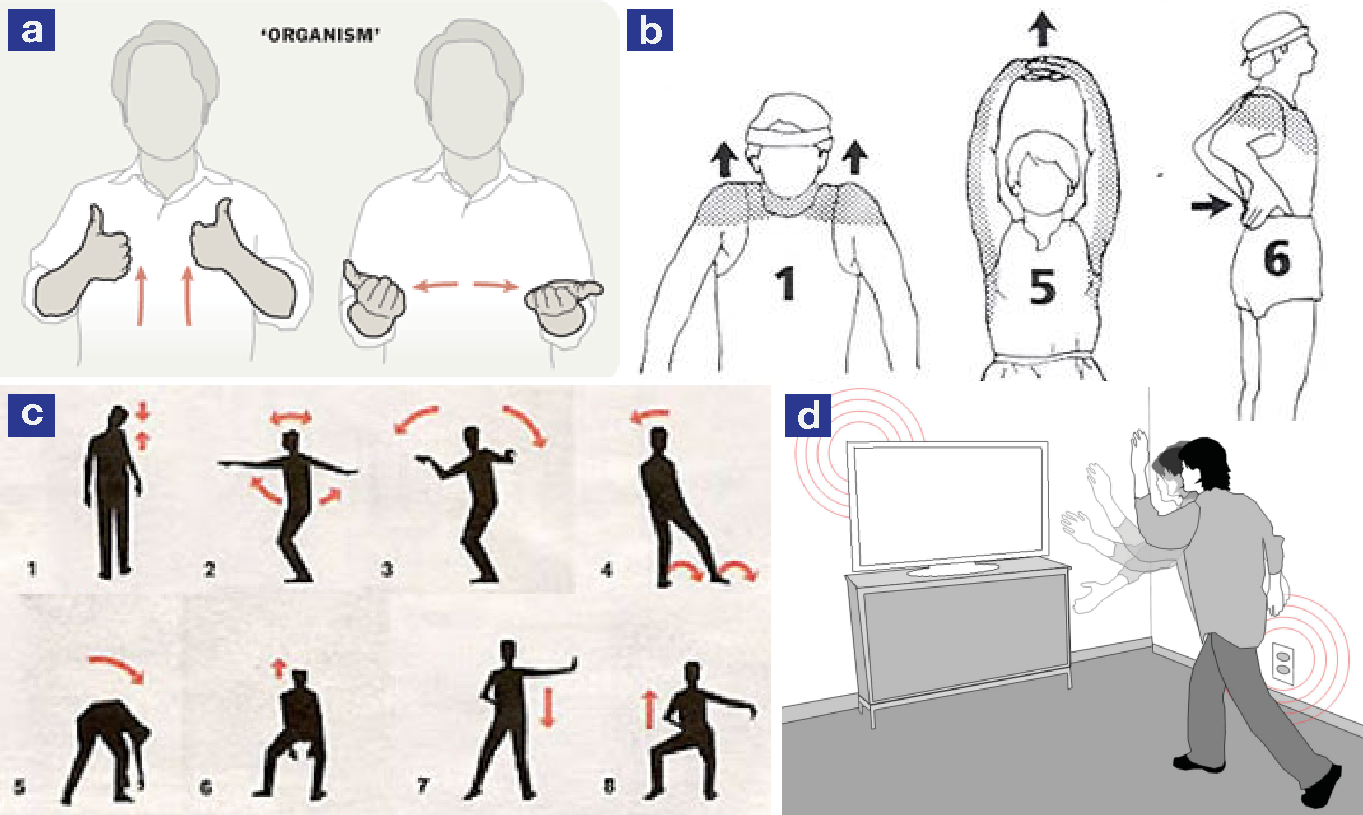
\includegraphics[width=0.6\columnwidth]{\demodraw/fig/existing_examples/existing_examples}
  \caption{Examples of manually generated human movement illustrations: (a) for sign language~\protect\cite{corum:2012:sign}; (b) for weight training~\protect\cite{anderson2010stretching}; (c) for dance steps [unknown]); (d) for a gestural interface~\protect\cite{cohn2012humantenna}.}
  \label{fig:existing_examples}
\end{figure}

We found that both professionals and non-designers create these kinds of illustrations, but the methods they use are commonly time-consuming and not amenable to iteration and editing.
It can take between 10 minutes and several hours to construct scenes, pose and take photos, trace them, and adjust details like arrow placement. Moreover, identifying the appropriate pose and viewpoint ahead of time can be difficult. One may choose to better orient or exaggerate hand motion after seeing the depiction. Unfortunately, changing these elements often requires starting over again with new source photos.
% it would be nice to add a more concrete example where capturing another source photo is necessary. e.g., a situation where the author realizes a more exaggerated motion would be better after seeing what the illustration looks like.

% Researchers have developed algorithms to visualize human motion~\cite{bouvier2007motion,choi2012retrieval,Assa2005action,assa2008motion}, but most prior work focuses on transforming datasets of pre-recorded motion capture sequences into visualizations for specific poses, not on authoring visualizations interactively.
% We extend an approach used in demonstration-based animation systems~\cite{Barnes:2008:VideoPuppetry,held20123d,Gupta:2014:MotionMontage} where demonstration and authoring are integrated into one interactive workflow.
% %
% However, in these systems users manipulate proxy objects to drive the animation of non-human objects and characters, usually with low degrees of freedom.
%
%To our knowledge, our system is the first to leverage full-body demonstrations of complex, high-degree-of-freedom motions to generate illustrated motion diagrams.

%a combination of these approaches -- visualizing full-body human motions from author's physical demonstration -- is yet a challenge, especially for a sequence of complicated movements.
% \peggy{I changed this to argue about the complexity of human motion performance}
% Authoring motion illustrations by demonstration is more challenging since the mapping from body movements to static illustrations conveying those motions is less direct. \bjoern{I don't understand the prior two sentences. What is directly about the mapping? How does it compare? Probably too complex to describe here.}

% Demonstration-based systems~\cite{Bergman:2005:DocWizards,grabler2009generating,chi2012mixt,chi2013democut} transform  demonstrations like screen recordings or video tutorials
% A common approach in graphics research is to generate illustrations \cite{agrawala2003designing} and mechanical work \cite{li2008automated, mitra2010illustrating} by analyzing object compositions. However, human motions involve degrees of freedom in a continuous space that can be difficult to decompose.
%\dan{Not sure the two sentences are motivating our work. In fact, \systemname{} does decompose human motion.}

% Commercial depth sensors can capture motion data and drive applications such as avateering [ref] and pose correction \cite{anderson2013youmove}. We leverage these capabilities with a hybrid method combining sensing, avateering, rendering, and user interaction would enable a new creation process of body-centric illustrations.
% \dan{I tweaked the sentences above, but I don't know if we really even need them.}

We propose \systemname{}, a system to enable people to rapidly create step-by-step motion illustrations through physical demonstration (see Figure~\ref{fig:teaser}). DemoDraw uses iterative demonstrations (with additions, re-takes, and refinements) as a first-class interaction method for authoring. This design serves two purposes: First, depicting motion arrows from source photos can be challenging. A demonstration-based approach allows authors to perform motions while our system automatically renders the character and arrows. Second, adjustments on initial depictions are commonly made. Supporting iteration in the creation workflow is critical.

Authoring proceeds in two modes: {\em Demonstration}, performed using body motions and voice commands; and {\em Refinement}, which uses a desktop interface.
% \peggy{Here I summarize our proposed method, but we can probably leave these details to the DemoDraw section}
%
The user first physically demonstrates desired motions in front of a Kinect RGB-D sensor. As in current instructional practice, they simultaneously speak during important parts (e.g., teaching dance moves with ``one, two, three, four'').
The motions are then mapped to a 3D human avatar rendered as a black-and-white contour drawing, a common style identified in our survey of illustration practices.
% \bjoern{Why? give the reason for preferring a line drawing or other simplified view.}
% \systemname{} captures the RGB-D information and logs the location and orientation data of her whole body with 25 joints in a 3D space. It then maps the data to a 3D humanoid avatar and applies Non-Photorealistic Rendering (NPR) effect to create line illustrations.
%
An algorithm analyzes speech and motion streams to segment motions into illustration figures with key frames. Salient joint movements are automatically identified and rendered as motion arrows overlaid on the stylized body drawing (Figure~\ref{fig:DemoDrawUI}c).
%
With this {\em \phaseI{}}, segmented motions can be reviewed and re-recorded using speech commands.
In addition, the annotation style and placement can be adjusted, camera angles moved, and alternate visualization styles explored in a mouse-driven GUI \emph{\phaseII{}} (see Figure~\ref{fig:DemoDrawRefinementUI}a).
% These visual parameters include rendering (outline, silhouette, or hybrid with an image background), arrow appearance, motion type (absolute positions, relative positions to a joint, or circular movement), and overlaying .
%\systemname{} also offers direct manipulation on the annotations, where the user can reposition the rendered arrows.
% \dan{I reduced description of \phaseII{} since it isn't the main contribution}
%
A three-part evaluation with 14 participants shows that \systemname{}'s illustrations are effective and amateur authors can use the \phaseI{} and \phaseII{} to proficiently create illustrations of movements with various levels of complexity.
% The generated illustrations were concise and expressive that provided only the necessary details with a similar visual style. Results from an online questionnaire with M feedback suggested that viewers preferred our system-generated illustrations over video recordings and annotated images (over a 5-Likert scale). An onsite user study with N participants showed that ...

DemoDraw integrates physical demonstration and authoring into one interactive workflow. Our work is the first to generate human movement illustrations by demonstration, refinement, and editing as an iterative process. Specifically, we make the following contributions:
\begin{itemize}
  % \itemsep -2pt
  \item An approach to generate human movement illustrations by direct physical demonstration and interactive rendering.
  \item Multi-modal interaction techniques to record, review, retake, and refine demonstration sequences.
  \item Methods to automatically analyze 3D motion data with speech to generate step-by-step annotated illustrations.
\end{itemize}

% -- Rebuttal --
% Our work contributes a functioning system leveraging multimodal interaction techniques to author illustrations by direct physical demonstration. To our knowledge, this is the first attempt at such a performance-based illustration system. We will clarify that we target non-experts who cannot effectively or efficiently illustrate motions using existing tools: our approach with interactive rendering techniques is a novel way to quickly communicate a sequence of movements. Like other systems research, the final product may appear somewhat obvious in hindsight, but it required a thorough understanding of the domain, many design iterations, and solving challenging technical problems.
